
\documentclass[12pt]{article} 
\usepackage[utf8]{inputenc}
\usepackage[slovak]{babel}
\usepackage[hidelinks,unicode = true]{hyperref}
\usepackage{outline}
\usepackage{graphicx}
%\usepackage{biblatex}
%\addbibresource{literatura.bib}
\usepackage{cite}
\usepackage{caption}
\setcounter{secnumdepth}{3}
\setcounter{tocdepth}{3}

%===========================================================================
\begin{document}           % Konec preambule a zároveň začátek vlastního textu
\begin{titlepage}
\centering
\Large \textbf{České vysoké učení technické v Praze }\\ Fakulta stavební
\vspace{2cm}

\begin{figure}[h!] %logoCVUT
\centering
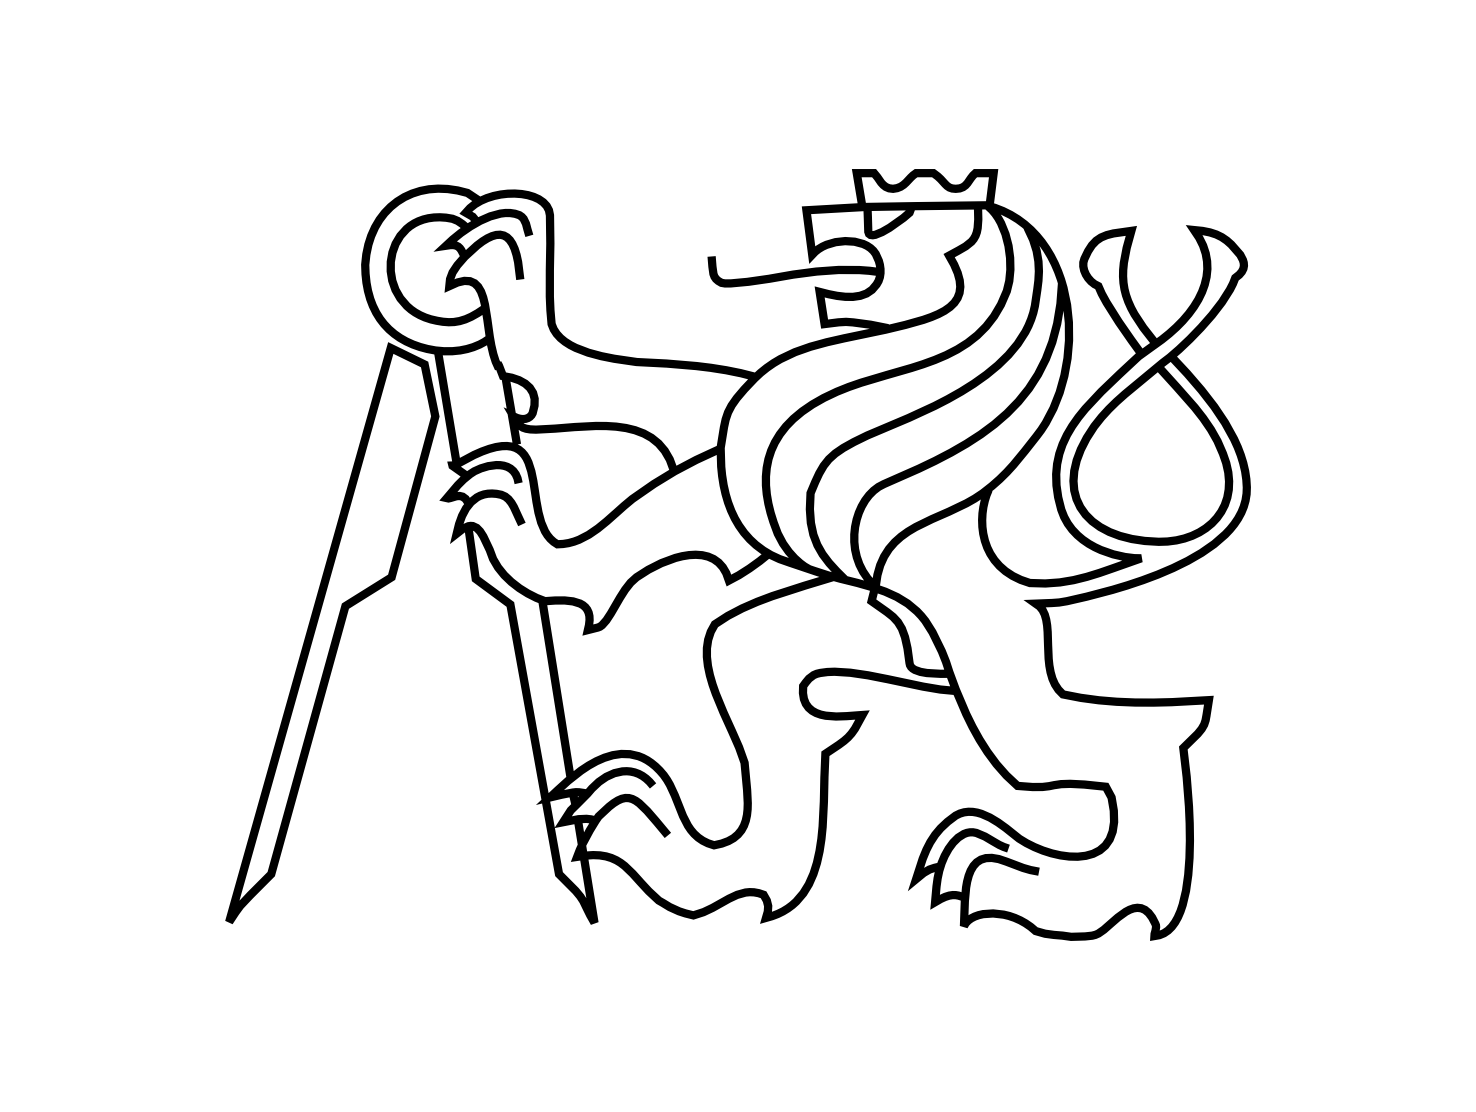
\includegraphics[width=7cm]{./img/cvut.png}
\end{figure}
 
\Large \textbf{155ADKG Algoritmy v digitální kartografii}
\vspace{1cm}

\LARGE  \textbf{ Konvexné obálky a ich konštrukcie}
\vspace{3cm}

\Large Bc. Lukáš Kettner Bc. Martin Hulín \\ 3.11.2019

 \thispagestyle{empty} %neočísluje první stránku
\end{titlepage}

\tableofcontents    % vytváří  Obsah 
\newpage %začne na nové stránce
%------------------------------------------------------------------------
\section{Zadanie}
Vytvorte aplikáciu s grafickým rozhraním, ktorá vygeneruje konvexnú obálku podľa zvoleného typu algoritmu. Vstup do aplikácie : množina bodov  \{p1, …, pn\} . Výstup aplikácie : konvexná obálka  \textit{H}(P).

Nad množinou   \textit{P} implementujte nasledujúce algoritmy pre konštrukciu \textit{H}(P).

\begin{itemize}
\item Jarvis Scan
\item Quick Hull
\item Sweep Line
\end{itemize}
		
Vstupné množiny vrátane vygenerovaných konvexných obálok vhodne vizualizujte. Vytvorte grafy pre množiny n $\in$ $\langle$ 1000, 1000 000 $\rangle$ ilustrujúce doby behu algoritmu. Meranie prevádzajte pre rôzne typy množín opakovane 10x a uvedťe rozptyl. Namerané údaje usporiadajte do tabuliek.

Taktiež sa zamyslite nad problémom singularít pre rôzne typy vstupných množín a nad možnými optimalizáciami. Zhodnoťte dosiahnuté výsledky. Rozhodnite, ktorá z týchto metód je vzhľadom na časovú náročnosť a typ vstupnej množiny najvhodnejšia.

\subsection{Bonusové úlohy}
V rámci úlohy sú vypracované tieto bonusové úlohy

\begin{itemize}
\item Konštrukcia konvexnej obálky metódou Graham Scan.
\end{itemize}
%------------------------------------------------------------------------

\section{Popis a rozbor problému}
Konvexná obálka je skupina bodov, ktorých spojením vznikne ohraničenie pre všetky ostatné body množiny. Pre konvexnú obálku platí : 

\begin{itemize}
\item žiadny bod vstupnej množiny \textit{P} neleží mimo ohraničenia konvexnej obálky.
\item všetky spojnice bodovvstupnej množiny \textit{P} ležia vnútri konvexnej obálky alebo tvoria jej ohraničenie.
\item všetky vnútorné uhly medzi susednými segmentami konvexnej pbálky sú menšie ako 180 stupňov.
\end{itemize}

\begin{center}
   \includegraphics[width=6cm]{./img/ch_obrazok1.png}
   \captionof{figure}{Princím konvexnej obálky}
\end{center}

Konvexnú obálku je možné zostrojiť viacerými metódami. V rámci našej práce sme zostrojili algoritmus Jarvis Scan, Quick Hull, Sweep Line a Graham scan.

%------------------------------------------------------------------------

\section {Popis použitých algoritmov}
\subsection {Jarvis Scan}
Tento algoritmus predstavuje jeden z najpoužívanejích postupov pre tvorbu konvexnej obálky. V algoritme sa zavádza kritérium maximálneho uhlu ($\omega_{max}$). Pri tomto kritériu posudzujeme uhol medzi poslednou stranou konvexnej obálky a úsečkou posledný bod obálky - aktuálny bod. Kritérium hladá taký aktuálny bod, pre ktorý je uhol ($\omega$) maximálny. 
Postup je nasledovný. V prvom kroku vyberieme pivot q so súradnicou $y_{min}$, tento bod je automaticky súčasťou konvexnej obálky. Zavádzame kritérium maximálneho uhlu ($\omega_{max}$). Keď nájdeme bod odpovedajúci kritériu, prídáme takýto bod do konvexnej obálky. Algoritmus končí v momente keď sa dostaneme opäť k pivotu q. 

\subsubsection {Implementácia metódy}
\begin{enumerate}
\item Nájdi pivot q. Zoraď body podľa súradnice y. $ q : y_{min}$
\item Do konvexnej obálky pridaj $q$
\item Inicializuj  $p_{j-1} \in X, p_j = q, p_{j+1} = p_{j-1}$
\item Opakuj pokial $p_{j+1} != q$
\item \hspace {1.5cm} Nájdenie bodu pre ktorý je uhol omega maximálny $p_{j+1} = argmax_{pi \in P} \angle(p_{j-1}, p_j, p_i)$
\item \hspace {1.5cm} Pridaj nájdený bod  $p_{j+1}$ do konvexnej obálky
\item \hspace {1.5cm} Inicializuj $p_{j-1} = p_j , p_j = p_{j+1}$ 
\end{enumerate}

\begin{center}
   \includegraphics[width=10cm]{./img/ch_obrazok1.png}
   \captionof{figure}{Princím konvexnej obálky}
\end{center}

\subsubsection {Problematické situácie}
Problematickou situáciou sú vyskytujúce sa kolineárne body. V takomto prípade je potrebné ošetriť aby sa do konvexnej obálky dostal najvzdialenejší bod.

\subsection {Quick Hull}
Tento algoritmus uplatňuje pri konštrukcii konvexnej obálky princím rozdeľuj a panuj. Jedná sa rekurzívny algoritmus. Skladá sa z lokálnej a globálnej procedúry. Konvexná obálke je skonštruovaná z dvoch častí - upper hull a lower hull. Deliacou priamkou je spojnica dvoch bodov s extrémnymi súradnicami x (minimum, maximum). S oboma časťami obálky sa počas výpočtu pracuje samostatne. Algoritmus hľadá bod s extrémnymi súradnicami v ose y, samostatne pre hornú a dolnú časť. Výsledná konvexná obálka je pri zachovaní CCW orientácie zložená z dvoch častí automaticky, bez nutnosti spájania.

\subsubsection{Implementácia metódy}

\begin{enumerate}
\item Tady něco bude
\end{enumerate}

\subsubsection{Problematické situácie}

\subsection {Sweep Line}
Jedná sa o metódu zametacej priamky. Tento algoritmus pracuje na princípe prepisovania pozície predchodcu a následníka i-teho bodu. Popis algoritmu slovne je miestami zložité pochopiť a pri jeho prezentácii pred osobou mimo obor by sme mohli skončiť na psychiatrii. Implemntácia metódy jednoduchšie zobrazí jej fungovanie.

\subsubsection{Implementácia metódy}
\begin{enumerate}
	\item  Zoradenie množiny bodov $P_s$ podľa súradnice x
	\item if $p_3 \in \sigma_L (p_1, p_2)$
	\item \hspace {1.5cm} n[1] = 2; n[2] = 3; n[3] = 1
	\item \hspace {1.5cm} p[1] = 3; p[2] = 1; p[3] = 2
	\item else
	\item \hspace {1.5cm} n[1] = 3; n[3] = 2; n[2] = 1
	\item \hspace {1.5cm} p[1] = 2; p[3] = 1; p[2] = 3
	\item for $p_i \in P_s, i > 3$
	\item \hspace {1.5cm} if ($y_i>y_i-1$) 
	\item \hspace {2.5cm} p[i] = i-1; n[i] = n[i-1]
	\item \hspace {1.5cm} else 
	\item \hspace {2.5cm} n[i] = i-1; p[i] = p[i-1]
	\item \hspace {1.5cm}n[p[i]] = i; p[n[i]] = i;
	\item \hspace {1.5cm}while (n[n[i]]) $\in \sigma_R (i, n[i]) $
	\item \hspace {2.5cm} p[n[n[i]]] = i; n[i] = n[n[i]];
	\item \hspace {1.5cm} while (p[p[i]]) $\in \sigma_L (i, p[i]) $
	\item \hspace {2.5cm} n[p[p[i]]] = i; p[i] = p[p[i]];
\end{enumerate}
\subsubsection{Problematické situácie}

\subsection {Graham scan}
Grahamov prehľadávací algoritmus využíva kritérium pravotočivosti, pri ktorom posudzuje uhol  ($\omega_i$). Množina bodov je zoradená podľa súradnice y. Bod s najmenšou y súradnicou je zvolený za pivota. Z pivota vedieme rovnobežku s osou X. Následne určíme uhol od osi X k ostatným bodom množiny. Tieto uhly je potrebné zotiediť podľa veľkosti. Následne vyberieme bod  ($p_i$) pre ktorý je uhol  ($\omega_i$) maximálny. Pri pridávani bodu do konvexnej obálky musí byť splnená podmienka ľavotočivosti.

\subsubsection{Implementácia metódy}
\begin{enumerate}
	\item Zoradenie množiny bodov $P_s$ podľa súradnice y 
	\item Nájdenie pivota q, $ q = min(y_i)$ , q $\to$ Convex Hull
	\item Zoraď body podľa veľkosti uhlu  ($\omega_i$) $ \angle(p_{kolinear} by x, x, p_i)$
	\item Vymaž bližší bod ku q $ if(\omega_i = \omega_j) $
	\item Opakuj pre všetky body j < n
	\item Pridaj bod $p_j$ pre ktorý je uhol omega maximálny a je splnená podmienka ľavotočivosti  $\to$ Convex Hull
	\item \hspace {1.5cm} j = j+1
	\item Else pop S	
\end{enumerate}

%------------------------------------------------------------------------

\section{Vstupné dáta}
Vstupnými dátami je množina bodov. Táto množina môže byť ručne naklikaná v Canvase alebo automaticky generovaná.
\subsection{Množina bodov}
Typy zadania množiny bodov : 

\subsection{Množina bodov vytvorená ručne}
Táto množina vznikne ručným naklikaním bodov priamo v Canvase.

\subsection{Automaticky generovaná množina bodov}
Množina vznikne automatickým vygenerovaním po zadaní požadovaného počtu generovaných bodov.

\section{Ukážka vytvorenej aplikácie}




%-------------------------------------------------------------------------

\section{Vykreslenie konvexnej obálky}



%-------------------------------------------------------------------------

\section{Dokumentácia}
\subsection{Trieda Algorithms}
Triedu Algorithms sme použili pre deklarovanie funkcií pre výpočtové algoritmy tvorby konvexnej obálky a pre deklaráciu ich pomocných metód.

\subsubsection{Metódy}

\begin{enumerate}
\item[] \underline{getAngle2Vectors}
\begin{itemize}
\item je pomocnou metódou pre metódu positionPointPolygonWinding. Slúži k určeniu uhlu medzi dvoma priamkami. Jej návratovou hodnotou je double
\item na vstupe má : súradnice bodov $p_1, p_2, p_3, p_4$ určujúcich prvú a druhú priamku
\item výstupom je hodnota uhlu medzi priamkami 
\end{itemize}

\item[] \underline{getPointLinePosition}
\begin{itemize}
\item je pomocnou metódou pre metódu positionPointPolygonWinding. Slúži na určenie polohy bodu voči priamke. Jej návratovou hodnotou je integer.
\item na vstupe má : súradnice určovaného bodu q , súradnice bodov priamky $p_1$ $p_2$
\item na výstupe hodnoty :
\item[] -1 – bod sa nachádza na priamke
\item[] 0 – bod sa nachádza vpravo od priamky
\item[] 1 – bod sa nachádza vľavo od priamky
\end{itemize}
\end{enumerate}

\subsection{Trieda Draw}
Trieda Draw slúži ku grafickému vykresleniu bodu q a konvexnej obálky.

\subsubsection{Členské premenné}



\subsubsection{Metódy}
\begin{enumerate}
\item[] \underline{paintEvent}
\begin{itemize}
\item slúži k vykresleniu zisťovaného bodu, vykresleniu importu polygónovej mapy a k vyfarbeniu polygónov ktorým náleží určovaný bod q. Návratovým typom je void.
\end{itemize}
\item[] \underline{void mousePressEvent}
\begin{itemize}
\item slúži k vykresleniu bodu q stlačením tlačidla myši, v okamihu stlačenia tlačidla na myši sa uložia súradnice bodu q. Návratovým typom je void.
\end{itemize}
\item[] \underline{void clearCanvas}
\begin{itemize}
\item slúži k vymazaniu obsahu vykreslovacieho plátna. Návratovým typom je void.
\end{itemize}
\end{enumerate}

\subsection{Trieda Widget}
Tieda Widget obashuje metódy ktoré sú odkazom na sloty umožňujúce vykonávať príkazy z grafického rozhrania aplikácie. Nemajú žiadne vstupné hodnoty, návratovým typom je void.

\subsubsection{Metódy}
\begin{enumerate}
\item[] \underline{on\_clearButton\_clicked}
\begin{itemize}
\item tlačidlo Clear, vyčistí grafické okno Canvasu
\end{itemize}
\end{enumerate}

%-------------------------------------------------------------------------

\section{Záver}

%-------------------------------------------------------------------------
\nocite{*}
%\printbibliography
\bibliography{literatura}{}
\bibliographystyle{plain}
%-------------------------------------------------------------------------
    
\end{document}             % Konec dokumentu.
